\chapter{Caching incident radiance}
\label{chapter:irradiance_caching}
The main goal of this thesis is to approximate the irradiance across a scene using local caches. Opposed to irradiance caching (as described in chapter \ref{irradiance caching}, \cite{ward}), where all the irradiance at one point is cached in one single value, we want to cache the incident radiance for different directions.\\
This chapter will cover all relevant preprocessing steps: Choosing a cache representation, placing the caches in the scene, and filling them. The next chapter will cover the actual rendering process and describe how these caches can be used in a path tracer to importance sample the irradiance.\\
We will use the term \textbf{IRC} (incident radiance cache) to refer to a cache.

\section{Environment Map Parameterization}
\label{envmap param}
Every IRC at a certain surface point is represented by a small local environment map. Every texel of this environment map will contain the relative incident radiance around the cache's position from the direction covered by that texel.

We chose the Octahedron representation proposed by \cite{octahedronpaper}. The main advantage of this parameterization is that in comparison to cube maps and especially sphere maps, all texels cover roughly the same solid angle. Since all probabilities in our path tracing algorithm are measured over solid angles, this choice results in the least distortion when converting probabilities between texel space and solid angles. This conversion is explained in chapter \ref{solidAngleConversion}.

Plus, the conversions between directions and texels are rather simple:\\
To map a direction $d=(d_x,d_y,d_z)$ on a texel coordinate $p = (p_x,p_y)$, we first use planar projection to convert the direction vector to a point on the unit octahedron surface:

\begin{equation}
d' = \frac{d}{|d_x| + |d_y| + |d_z|}.
\label{planar_projection}
\end{equation}

Next we need to project this point on a two-dimensional texture coordinate $p$. There are several ways to do this, we chose one that yields a rectangular texture: 

\begin{equation}
p = \begin{cases}
  (d_x' - d_z' - 1, d_x' + d_z')  & \text{ } d_y' \geq 0 \\
  (d_z' - d_x'+ 1, d_x' + d_z') & \text{ } d_y' < 0.
\end{cases}
\label{planar_projection2}
\end{equation}

\begin{figure}[ht]
	\centering
\def\svgwidth{230pt}
\input{planar_projection.pdf_tex}
	\caption{Planar Projection}
\label{texture_coord}\end{figure}



Figure \ref{texture_coord} depicts the complete projection. The resulting coordinate lies in $\left[-2,2\right]\times\left[-1,1\right]$, with directions of the upper hemisphere being mapped to $\left[-2,0\right]\times\left[-1,1\right]$ and directions of the lower hemisphere being mapped to $\left[0,2\right]\times\left[-1,1\right]$. As seen in figure \ref{octamap}, texels close to $p_x = 0$ belong to similar directions on adjoint octahedron surfaces. 

\begin{figure}[ht]
	\centering
	\def\svgwidth{230pt}
  \input{octahedronmap.pdf_tex}
	\caption{The upper hemisphere is mapped to the left side, while the lower hemisphere (if needed) is mapped to the right half.\newline
The borders in the final map match the octahedron edges.}
	\label{octamap}\end{figure}


This projection is relatively easy to calculate back and forth, plus the resulting texels cover the whole area of the texture. Since both hemispheres are mapped to separate parts of the texture we can simply ignore the lower hemisphere at non-transmitting surfaces, when irradiance from below has no contribution to the outgoing light. We can then only use radiance arriving at the upper hemisphere by only using - and storing - the left half of the environment map, which also saves a considerable amount of storage space.

\section{Creating Caches}
Actually creating these caches consists of 4 steps: Photon Mapping, distributing the positions of the caches over the scene, filling the caches and storing them.\\
Since we intend to fill the caches with incident radiance, we need some way to approximate it. We do this with a modified version of photon mapping. When the photon mapping is done, the photons are used to place and fill the caches.



\subsection{Modified Photon Mapping}
\label{modified photon mapping}
The idea of photon mapping is to trace a huge number of emitted photons from all light sources along their paths and store a photon at every surface point along that path. Originally, the resulting photon map would then be used to render the image. We give a short introduction on photon mapping as a stand-alone rendering technique in chapter \ref{photon mapping}.

\newpage
\textbf{Creating a photon path}

A photon path is initialized by sampling a point and outgoing direction for a photon and then tracking it across the scene. Whenever there are multiple light sources, a light source $L$ is chosen with a probability $p_L$ proportional to its surface area $A_L$ and its flux $\Phi_L$: 

\begin{equation}
p_L = \frac{A_L \cdot \Phi_L}{\sum_{L'}A_{L'} \cdot \Phi_{L'}}.
\end{equation}

For simplicity's sake we only consider area light sources here. A point $x$ on light source $L$ is sampled uniformly with probability $p_x = 1/A_L$, the probability for sampling direction $\omega_o$ at this point is $p_\omega$. Given a light source L, let $L_e(x,\omega_o)$ be the power of that light source for the given origin $x$ and direction $\omega_o$. When $N$ photons are emitted, the initial energy of the photon emitted from light source $L$ at $x$ into $\omega_o$ is given as

\begin{equation}
\label{initialenergy}
\frac{L_e(x,\omega_o)}{p_L \cdot p_x \cdot p_\omega \cdot N} =  \frac{L_e(x,\omega_o)}{p_\omega} \cdot \frac{\sum_{L'} A_{L'} \Phi_{L'}}{\Phi_L \cdot N}.
\end{equation}


This photon is then traced across the scene. Whenever the photon's path intersects a diffuse surface, a photon with the current energy is stored. At any intersection $y$, no matter if it's diffuse or specular, the outgoing direction $\omega_o$ of the photon path is sampled from the surface's adjoint (see \ref{BSDF}) BSDF and the incoming direction $\omega_i$. The path is continued into the sampled direction and the energy is weighed with the BSDF's value $f_s(\omega_i,y,\omega_o)$ divided by the probability of sampling $\omega_o$.\\

\textbf{Adjustments for IRCs}

Since we plan to use photon mapping to approximate incident radiance instead of rendering an image we need to make some adjustments to this process. One of them are the stored photons themselves: Each of our photons consists of its position including the local surface coordinate system, its incoming direction, a pointer to the surface's BSDF and its energy. The next section will explain why the local coordinate system is necessary. The BSDF is needed in case we want to place a cache at the photon's position: It tells us whether we need an environment map for both hemispheres or only one. We don't need the actual energy distribution over different wavelengths; storing a photon's average energy in a single float value is sufficient.

Besides, we only need the relative incident radiance from all directions to create a cache. This allows us to ignore the constant factors in \ref{initialenergy} (the fraction on the right) when computing a photon's initial energy; we can use 

\begin{equation}
\frac{L_e(x,\omega_o)}{p_{\omega}}
\end{equation}
 
 instead. To avoid unnecessary computing, we cancel photon paths when their accumulated energy falls too close to zero, when the path length reaches 32 and using Russian Roulette. As soon as all photon paths are complete, all created photons are stored in a k-d tree (\cite{kdref1}, \cite{nanoflann}).


\newpage

\subsection{Placing Caches}
\label{placing caches}
There are two interesting areas for placing IRCs: Those with much incident light, and those that are potentially hit very often when using path tracing later on.

To cover the latter, we send a camera ray through the upper left corner in every $8\times 8$ pixel block. If the BSDF at its first intersection with the scene is smooth, we place a cache at that position. Otherwise the ray will be traced until it leaves the scene or until a surface with a smooth BSDF is hit so we can place a cache. We call the resulting caches \emph{camera caches}.

The remaining cache positions are adopted from the first $n$ photon positions from the photon mapping step. This will lead to many caches in areas where many photons arrive, and place less caches in areas where only few photons intersect the scene.  Since the photon paths were constructed randomly,  the distribution of cache positions generated from simply taking the first $n$ photons will  be similar (on average) to choosing the photons randomly.

Note that from now on we have almost no information concerning the surface properties (BSDF, geometry, normals) at the cache position. We only know the positions themselves and that they are placed at non-delta BSDFs. To avoid inconsistent coordinates later on, it is necessary to give each cache its local coordinate system. Luckily we already stored these systems with every photon and can simply use these for the photon caches. The camera caches get their coordinate system from the intersection information which is still available when the caches are placed in the scene.

At this point we also need to decide whether to create a cache for irradiance from both hemispheres or only one. To do so, we look at the BSDF (which is either stored in the photon or can be retrieved from the intersection information for camera caches): If it is transmitting, we create an empty environment map for both hemispheres and store it at the position with its coordinate system. Otherwise a map for the upper hemisphere is created and stored. Practically the only difference between these two IRCs is the length of the array containing the environment map's texels. We don't consider materials where only irradiance from below contributes to radiance leaving at the upper side.

\subsection{Filling a Cache}
After the caches are created and placed across the scene we need to fill them with an approximation of the incident radiance around them. The number $k$ of photons used to fill a cache is fix and can be adjusted before the image is rendered. Filling a cache works like this:
\newline
\begin{algorithmic}
\State $photon list \gets $ \Call{$kdTreePhotons.getKClosestPhotons$}{$k,cache.position$}
\ForAll{$Photon$ $p$ in $photon list$} 
	\State $incoming\_direction\_local \gets $\Call{$cache.transformToLocal$}{$p.direction$}
    \If {$cos(local\_incoming\_direction) > 0$ $||$ $cache\_for\_both\_hemispheres$}
        \State $texel \gets $ \Call{$cache.convertDirectionToTexel$}{$incoming\_direction\_local$}
        \State $cache.environmentMap\lbrack texel \rbrack += p.energy$
    \EndIf
\EndFor
\end{algorithmic}

Whenever a photon is deemed useful to fill a cache, its incoming direction is converted to a texture coordinate for our octahedron environment map (see equations \ref{planar_projection} and \ref{texture_coord}).

We found that filtering the caches considerably reduces the noise in the final image.
First we apply bilinear filtering to distribute the energy of each photon over the texel itself and its left/right, upper/lower and diagonal neighbour. This is done while the photons are added to the cache one by one.

After the cache has been filled, we use a Gaussian filter

\begin{equation*}
\frac{1}{16}\begin{pmatrix} 1 & 2 & 1 \\ 2 & 4 & 2 \\ 1 & 2 & 1 \end{pmatrix}
\end{equation*}

on all texels. In order to filter the texels on the edge, we simply added the texels from the opposite side. Theoretically, this is not correct, as texels on opposing edges may correspond to opposing directions (see figure \ref{octamap}). But the improvement on the images was big enough, so we stayed with that simplification.\\
We found that Gaussian filters showed a bigger improvement than bilinear filtering, and the combination of both could noticeably reduce the noise of an image, see figure \ref{filtervergleich}.\\

\begin{figure}[ht]
	\centering
  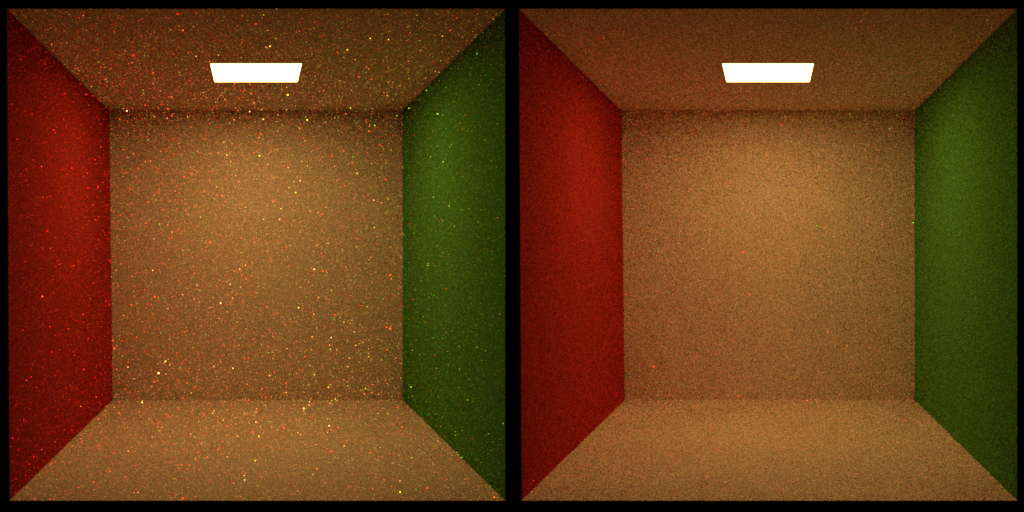
\includegraphics[width=1\textwidth]{bilder/filter/filtervergleich.png}
	\caption{Left: No filtering.\newline
Right: bilinear filtering and Gaussian filter.\newline
Both images were rendered with IRCs only (no BSDF sampling or NEE), using 150.000 photon paths ($\approx$ 750.000 photons), 20.000 caches, 500 photons per cache and 64 samples per pixel.}
	\label{filtervergleich}
\end{figure}



 We also tried to weight the energy contribution of a photon with its distance to the cache's position or with the Epanechnikov kernel \cite[chapter 8]{epanechnikov}. The difference was barely noticeable, but the images seemed a little better without these weights.

One last thing to note is that the number of photons actually contributing to a cache may be lower than $k$. Figure \ref{fill_cache_cos} illustrates an example.

\begin{figure}[ht]
	\centering
\def\svgwidth{250pt}
  \input{bilder/fill_cache_cos.pdf_tex}
	\caption{When filling the cache with 4 photons, photons p1 to p4 are considered and p5 is ignored. However, the incoming direction of p2 results in a negative cosine with the cache's surface normal, meaning that the photon arrives from below from the cache's point of view. Thus p2 is discarded for this cache and only p1, p3 and p4 are used to fill it.}
	\label{fill_cache_cos}
\end{figure}


\newpage
\subsubsection{Creating a useful probability density function}
The next step is to convert the filled environment map to a probability density function that can be used to sample an outgoing direction proportional to the incident radiance during path tracing. The main idea is to normalize the sum of all texels of the environment map to 1 and then sample directions according to the probability values stored in the texels. Obviously, the first step towards a useful pdf is simply that: add up all energy values from the environment map and divide every texel's value by that sum.

However, we have to consider that Monte Carlo integration requires the pdf to be greater than zero wherever the integrated function contributes to the integral. So we have to make sure that our pdf isn't equal to 0 when radiance arriving from the corresponding direction can contribute to the integral. With non-delta BSDFs that is the case for all directions (in the upper hemisphere), so we have to set all texels with value 0 to a bigger value. This value should be big enough so it won't cause any floating point precision problems - either by being ignored completely in the final pdf or by causing fireflies due to dividing by very small numbers. On the other hand the value should not affect the quality of the radiance approximation stored in non-zero texels.

We tried several options: The first one was setting the zeros to the smallest positive value from all other texels before normalizing. However, in many cases this value turned out to be too close to zero and disappeared completely after the normalization. Even normalizing, setting all 0 texels to the smallest value after normalizing, and normalizing again resulted in near-zero values that didn't work well in the final image.\newline
Next we tried setting every value below half average of all non-zero values to half average. The reason for that idea was that many caches had some texels with values around some 100, but a lot more texels containing positive values below 1. This approach caused by far the most noise in the final image.\newline
After looking at several normalized environment maps, we tried to simply set all values smaller than 0.0002 to 0.0002 and normalize again. This seemed to be working quite well so far. We even tried combining this approach with the first one, but as it turned out the minimal value was always smaller than 0.0002, regardless of whether it was picked before or after the first normalization. Different thresholds from 0.0001 to 0.001 didn't produce any noticeable differences in the final images.

There's also a reason not to set every 0 to a fix non-zero value before the first normalization: The sums of two caches can easily differ in an order of 2 magnitudes. So while setting all 0 texels to, say, 1 may work perfectly fine for one cache with a (previous) sum of some 100, it can totally destroy the irradiance approximation for another one with a sum of 50 or just disappear again for caches in bright regions with sums up to some 1000. Additionally, the initial sum of a cache depends on the number of photons used to fill it and the overall energy of these photons, while the average value of a texel also depends on the resolution of the octahedron map. Considering all these uncertainties it seems more reasonable to increase the 0-texels after a first normalization, when we can make a more precise statement about the overall properties of the cache.

The values of the environment map now form a valid probability density function that can be used to sample directions. This pdf is currently measured over the texel space, where each texel covers a unit square and all texel values sum up to 1.\\
To improve computation time we also create a second environment map (the $cdf\_map$) containing the cumulative density function for that pdf and added it to the cache. See chapter \ref{path extension} on how samples are torn from these environment maps.

\newpage
\subsubsection{Convert probabilities to solid angle}
\label{solidAngleConversion}
Generating samples is not the only purpose of these caches. The other one is to get the probability linked to the sampled direction, and to compute the probability of sampling a given direction from a cache. These probabilities are needed to compute weights for Multiple Importance Sampling and to compute the probability of sampling a path.\\
While probabilities for path tracing are usually measured over solid angle, our pdf is measured over a rectangle (or square in case only the upper hemisphere is important). Its width and height correspond to the number of columns and rows of the environment map, and each texel covers the area of one unit square. Remember that the pdf values were normalized to sum up to one.

Unfortunately, there is no easy way to analytically compute the solid angle covered by each unit square in our environment map. Ignoring this problem and directly using the probability value from a cache resulted in almost completely white images. This is due to the fact that with a $16\times 16$ resolution, every pdf value is roughly $\frac{2\pi}{256}$ times as big as it should be. Thus the accumulated probability of sampling a certain path is several orders of magnitude smaller than the correct value, and dividing by it causes the energy to reach insanely high values.\newline
Approximating the solid angle measure by multiplying with $\frac{size\_of\_environmentmap}{2\pi}$ isn't enough either: The overall energy of the resulting images seemed about right, but it was rather weirdly distributed (see figure \ref{solid_angle_korrektur}). So we created another map to approximate the solid angle covered by each texel:
\newline
\begin{algorithmic}
\State $solid\_angle\_map \gets $new $octahedronMap$ \Comment upper hemisphere only
\State $numSamples \gets 1000 \cdot solid\_angle\_map.width \cdot solid\_angle\_map.height$
\For{$i = 0$ to $numSamples$}
	\State Vector3 $sample \gets $ $createRandomSampleOnHemisphere()$
	\State Vector2 $texel \gets $\Call{$solid\_angle\_map.convertDirectionToTextureCoordinate$}{$sample$}
	\State $index \gets \lfloor texel.x \rfloor + solid\_angle\_map.width ^* \lfloor texel.y \rfloor$
	\State $solid\_angle\_map\lbrack index \rbrack \gets solid\_angle\_map\lbrack index \rbrack + 1$
\EndFor
\For{($i=0$ to $solid\_angle\_map.length$)}
	\State $solid\_angle\_map\lbrack i \rbrack$ $/=numSamples$ \Comment normalize to 1
	\State $solid\_angle\_map\lbrack i \rbrack$ $^*= 2\pi$ \Comment integral over one hemisphere is $2\pi$
\EndFor
\end{algorithmic}

At the end every texel represents the relative solid angle covered by its area. Central texels and those close to the border represent directions close to the surface's normal and along the surface itself respectively and will hold smaller values. The areas in the middle of each octahedron surface are close to parallel to the unit hemisphere and thus cover a bigger solid angle. Figure \ref{solid_angle_map} shows the resulting maps for $4\times 4$, $8\times 8$ and $16\times 16$ texels, and figure \ref{solid_angle_skizze} depicts the relation between texel area and solid angle.

\begin{figure}[ht]
	\centering
  
\includegraphics[width=0.8\textwidth]{bilder/solid_angle_maps.png}
	\caption{Solid angle maps with $4\times 4$, $8\times 8$ and $16\times 16$ texels for one hemisphere}
	\label{solid_angle_map}
\end{figure}

\begin{figure}[ht]
\centering
\def\svgwidth{200pt}
\input{bilder/solid_angle_skizze.pdf_tex}
\caption{Solid angle areas covered by texels of different height for a 8x8 map. Texels on the octahedron surface's center (blue, green) cover a larger solid angle than those close to the surface (yellow) or at the top (red).\newline
Note that the difference between the texel values also depends on their horizontal distribution.}
\label{solid_angle_skizze}
\end{figure}

A pdf value from a texel in a cache's environment map can now be converted to a probability value measured over solid angle by dividing it by the value from the corresponding texel in the solid angle map. This can be done for all texels in all environment maps in a preprocessing step, as the number of accesses to caches during the actual rendering may easily exceed the total number of texels. \newline
The solid angle map can also be doubled and then applied to the lower hemisphere. In that case its values will sum up to $4\pi$, which equals the integral over the unit sphere.

\begin{figure}[h!]
	\centering
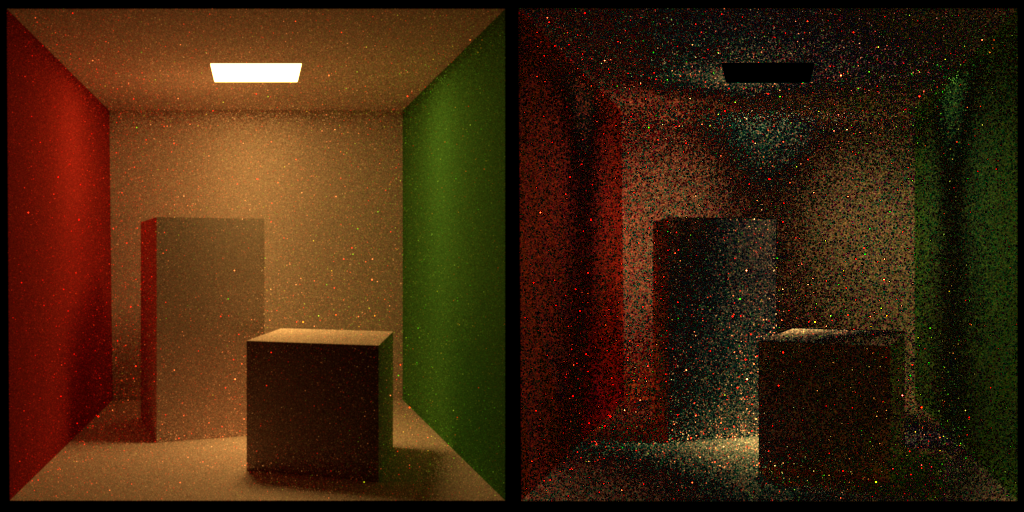
\includegraphics[width=1\textwidth]{bilder/solid_angle_difference.png}
\caption{Left: Solid angle correction with $\frac{width \cdot height}{2\pi}$\newline
Right: Difference with correct reference, multiplied by $4$. Note the vertical stripes on the wall in both images and the bright area in the middle of the floor.}
\label{solid_angle_korrektur}
\end{figure}

\clearpage
\subsection{Storing Cache}
\label{storing cache}
All caches are stored in a k-d tree (\cite{kdref1}, \cite{nanoflann}) for fast and easy access. The k-d tree containing the photons won't be needed again and can be deleted.
In the end, each IRC consists of the following components:
\begin{itemize}
\item An octahedron environment map containing the probability density function, measured over solid angle, that approximates the incident radiance around the cache. We will call this one the $pdf\_map$.
\item An additional map containing the cumulative density function for faster sampling, called $cdf\_map$. Note that the cdf is created after the last normalization, but before the pdf is adapted to the solid angle measure.
\item Its position.
\item Its local coordinate system.
\end{itemize}